%\documentclass[a4paper,12pt, draft]{report}                         %print on one side
\documentclass[a4paper,12pt,twoside,notitlepage,openright]{report} %print on both side


\usepackage[bookmarks=false, colorlinks=false,unicode]{hyperref}
\usepackage[abbr,dcucite]{harvard}      %style ofliterature
\usepackage{index}                      %make index
%\makeindex
\usepackage{Styles/COP}
%\usepackage{showframe}                  %show edges of pages (for oneside, comment line 
                                            %\setlength{\oddsidemargin}{5mm} in COP.sty)
%%%%% HERE PUT ALL THE RELEVANT PACKAGES


\usepackage{pdfpages} % pokud nemáte formulář "Zadání bak./dipl. práce" naskenovaný jako PDF, tak ZAKOMENTUJTE

% path for figures
\graphicspath{{img/}}

\usepackage{epigraph}
%\ setting the epigraph width
\setlength{\epigraphwidth}{0.8\textwidth}

\usepackage{graphicx} % balíček pro vkládání rastrových grafických souborů (PNG apod.)
%\usepackage{epsfig} % balíčky pro vkládání grafických souborů typu EPS
%\usepackage{float} % rozšířené možnosti umístění obrázků 

\usepackage{grffile}

% captions of figures
\usepackage[font=small,labelfont=bf,width=1.0\textwidth]{caption}

% csquotes for advanced quoting
\usepackage{csquotes}

% balíček pro vkládání rastrových grafických souborů (PNG apod.)
\usepackage{graphicx} 

\usepackage{tabularx} % rozšířené možnosti tabulek

\usepackage{amsmath} % balíček pro pokročilou matematickou sazbu

% for footnotes in tables
\usepackage{booktabs,caption}
\usepackage[flushleft]{threeparttable}

% for table footnotes and captions
\usepackage{caption}
%% \usepackage{subcaption}



% for printing of units
\usepackage{siunitx}
\sisetup{load-configurations = abbreviations}

% for printing of multiline comments
\usepackage{verbatim}

% package for simple quations
\usepackage{dirtytalk}

\usepackage{comment}

\usepackage[sorting=none]{biblatex}
\addbibresource{Refer.bib}



%-----<<<<<<<<<<<< NAMES NAD PATHS >>>>>>>>>>>>-----
\def \Bookname {Postprocesor robota pro metodu Laser Shock Peening}
\def \BooknameEN {Robot post processor for Laser ShockPeening technique}
\def \Author {Marek Böhm}
\def \Year {2022}




\def \APforPrint {0}

\def \BookName {ABSOLVENTSKÁ PRÁCE}
\def \HEAD {Vyšší odborná škola, Střední škola, Centrum odborné přípravy\\ Sezimovo Ústí}
\def \SCHOOL {Vyšší odborná škola, Střední škola,}
\def \FACULTY {Centrum odborné přípravy}
\def \Place {Sezimovo Ústí}

\def \cestaFiles {00_files/}
\def \cestaJedna {01_Intro/}
\def \cestaDva {02_Chapter2/}
\def \cestaTri {03_Chapter3/}
\def \cestaCtyri {04_Chapter4/}
\def \cestaPet {05_Chapter5/}
\def \cestaSest {06_Chapter6/}
\def \cestaZaver {05_Concl/}
\def \cestaAP {A_Appendices/}
\def \cestaStyles {Styles/}

\newindex{default}{idx}{ind}{Rejst\v r\'ik}

\newcounter{YearOld} \setcounter{YearOld}{\Year} \addtocounter{YearOld}{-1}
%-----<<< --------------------------------- >>>-----



%-----<<<<<<<<<<<< DOCUMENT >>>>>>>>>>>>-----
\begin{document}

%-----<<< BINDING >>>-----
%\iffalse
\pagestyle{empty}                       %no pagination
\input{\cestaFiles Binding.tex}         %input file
\cleardoublepage

%-----<<< ------- >>>-----


%-----<<< EMPTY PAGE - VAKÁT >>>-----
%\thispagestyle{empty}
\begin{verbatim}

\end{verbatim}
\cleardoublepage
%\fi
%-----<<< --------------------- >>>-----


%-----<<< TITLE PAGE >>>-----
\pagestyle{empty}                       %no pagination
\BookHeadDP
\cleardoublepage
\clearpage
%-----<<< ---- >>>-----


%-----<<< TASK AP >>>-----
\pagestyle{plain}                       %pagination
\pagenumbering{roman}                   %start roman pagination from 1
$ $
\input{\cestaFiles Task.tex}            %input file
\cleardoublepage
%-----<<< ------------------------- >>>-----


%-----<<< DECLARATION >>>-----
$ $
\input{\cestaFiles Declar.tex}          %input file
\newpage
%-----<<< ----------- >>>-----


%-----<<< ACKNOWLEDGEMENT >>>-----
$ $
\input{\cestaFiles Acknow.tex}          %input file
\newpage
%-----<<< --------------- >>>-----


%-----<<< ANNOTATION >>>-----
\input{\cestaFiles Annotation.tex}      %input file
\cleardoublepage
%-----<<< ---------- >>>-----


%-----<<< TABLE OF CONTENTS >>>-----
\setcounter{secnumdepth}{4}             %number of section to 4
\setcounter{tocdepth}{4}                %number of section in table of contents greater then 3
\tableofcontents
\cleardoublepage
%-----<<< ----------------- >>>-----


%-----<<< USABLE SYMBOLS >>>-----
% \input{\cestaFiles Symbols.tex}
% \cleardoublepage
%-----<<< ----------------- >>>-----


%-----<<< TABLE OF FIGURES >>>-----
\addcontentsline{toc}{chapter}{List of Figures}
\listoffigures
\cleardoublepage
%-----<<< ---------------- >>>-----


%-----<<< TABLE OF TABLES >>>-----
\addcontentsline{toc}{chapter}{List of Tables}
\listoftables
\cleardoublepage
%-----<<< --------------- >>>-----


%-----<<< CHAPTERS >>>-----
\pagenumbering{arabic}                  %start arabic pagination from 1
\hyphenation{Automatica}                %no divide words
\pagestyle{headings}
\setcounter{footnote}{0}

\input{\cestaJedna Intro.tex}           %input file
\input{\cestaDva Chapter2.tex}
\input{\cestaTri Chapter3.tex}
\input{\cestaCtyri Chapter4.tex}
\input{\cestaPet Chapter5.tex}
\input{\cestaSest Chapter6.tex}
\input{\cestaZaver Concl.tex}
%-----<<< -------- >>>-----


%-----<<< REFERENCES >>>-----
%\bibliograp
hystyle{\cestaStyles COP}
%\bibliography{\cestaStyles Refer,\cestaStyles Refer_BP}%references from BIBTEX
\addcontentsline{toc}{chapter}{Bibliography}
\printbibliography
% Biblatex package for references

%\iffalse

%\input{\cestaStyles Refer.tex}          %input file

%\fi
\newpage\thispagestyle{empty}
%-----<<< ---------- >>>-----



%-----<<< APPENDIXS >>>-----
\cleardoublepage
\addcontentsline{toc}{chapter}{Appendices}
\def\appendixname{Appendix}
\pagenumbering{Roman}                   %start arabic pagination from 1
\begin{appendix}
%% \addcontentsline{toc}{chapter}{Appendix A}
\input{\cestaAP AppendCD.tex}           %input file
\input{\cestaAP AppendSW.tex}           %input file
\input{\cestaAP AppendPlan.tex}         %input file
%% \input{\cestaAP AppendTime.tex}         %input file
%% \input{\cestaAP AppendBudget.tex}       %input file

%% TYTO TRI ODKOMENTOVAT, AZ S TIM BUDU DALE PRACOVAT

%\chapter[Stručný manuál pro \LaTeXe]{Stručný manuál pro tvorbu AP v~publikačním systému \LaTeXe \label{ch:Manual_tex}}


V~této příloze je stručně uvedeno, jak vkládat do publikačního systému \LaTeXe\/ základní objekty (kapitoly, obrázky, tabulky, citace, křížové odkazy, rovnice atd.). Sledujte zdro\-jo\-vé kódy (soubory {\rm \texttt{*.tex}}). Tento text se nachází v~souboru \texttt{\cestaStyles Manual\_tex.tex}.



\section{Obrázky a~tabulky}


\subsection{Obrázky}

Obrázky do LaTeXu vkládáme ve formátu \verb"*.eps", které ukládáme do příslušných podadresářů \texttt{Figures}. Můžeme vkládat obrázky samostatně nebo vedle sebe jako \uv{podobrázky}.

\begin{figure}[H]
\begin{center}
    {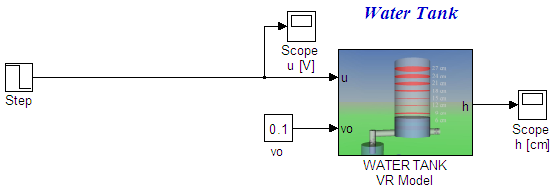
\includegraphics[height=4cm, angle=0]{\cestaStyles Figures/ModelWS}}
    \caption[Simulinkový model vodní nádrže -- převzato z~\protect\cite{Book:ROUBAL-HUSEK-kol_RTvP}]
        {Simulinkový model vodní nádrže -- převzato z~\protect\cite[Příloha\?: VR\_Toolbox\_Water.pdf]{Book:ROUBAL-HUSEK-kol_RTvP}}
    \label{fig:ModelWS}
\end{center}
\end{figure}

\begin{figure}[H]
\begin{center}
  \subfigure[napětí zubového čerpadla~$u$]
    {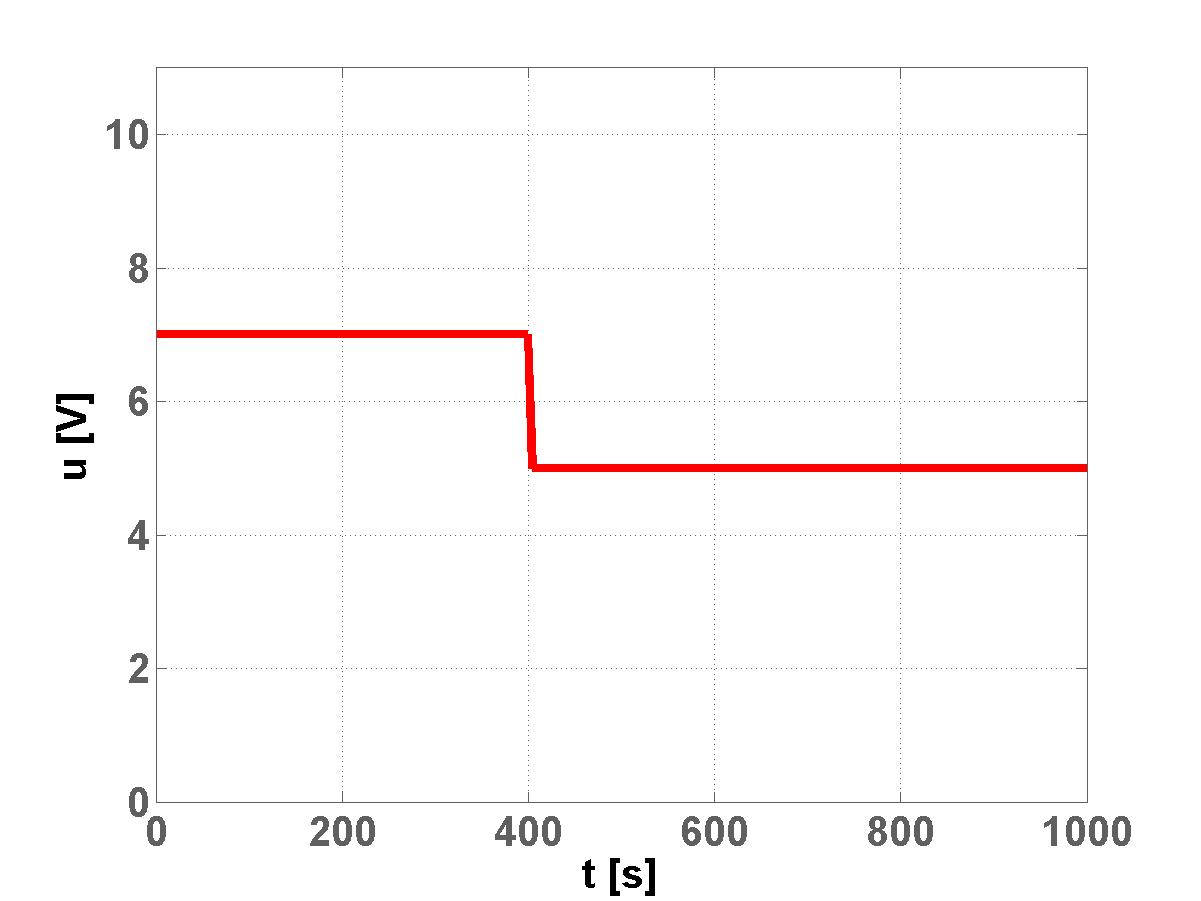
\includegraphics[width=7cm]{\cestaStyles Figures/Data_u}
    \label{fig:Data_u}}
  \hspace{1cm}
  \subfigure[výška hladiny v~nádrži~$h$]
    {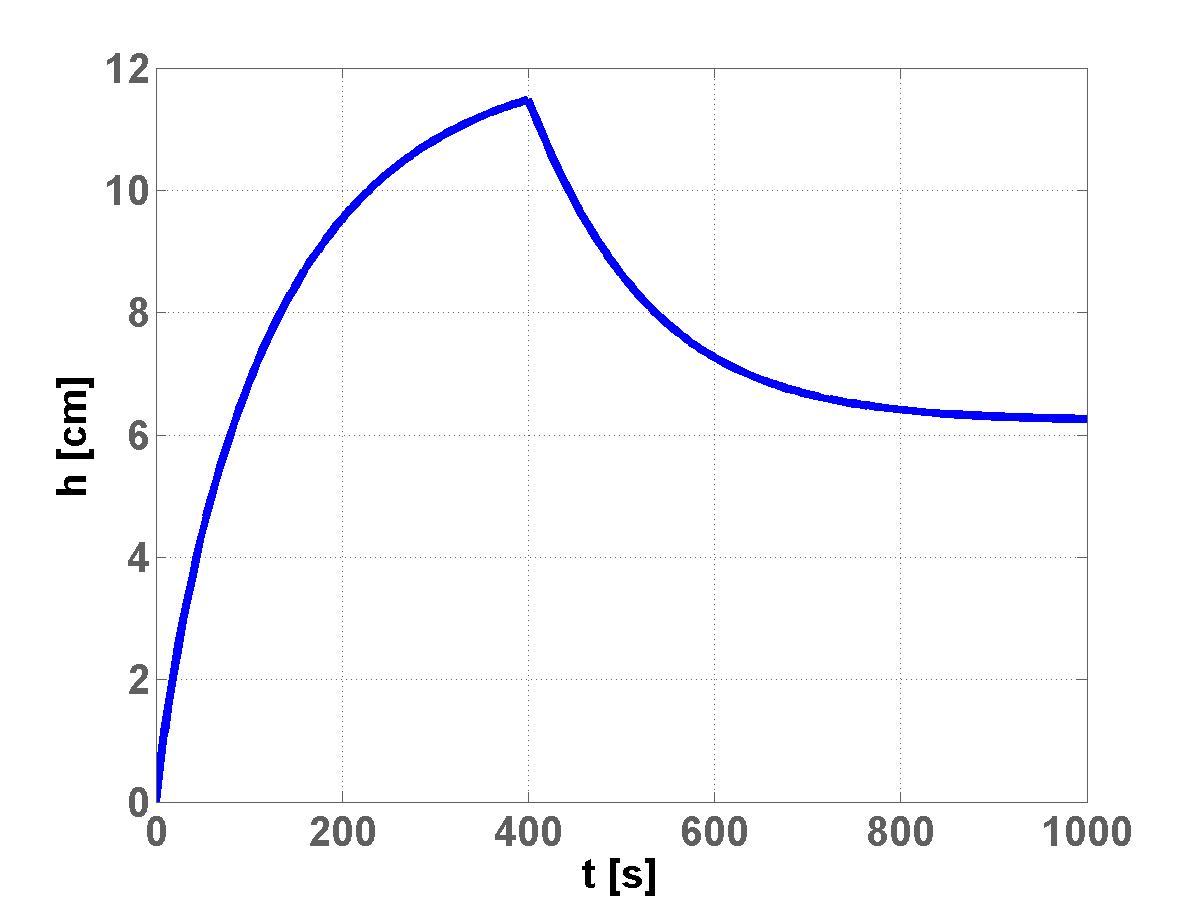
\includegraphics[width=7cm]{\cestaStyles Figures/Data_h}
    \label{fig:Data_h}}
  \caption[Časové odezvy virtuálního modelu vodní nádrže]
    {Časové odezvy virtuálního modelu vodní nádrže\protect\footnotemark}
  \label{fig:Data}
\end{center}
\end{figure}
\footnotetext{Obrázky převzaty
z~$\langle${\href{http://apps.copsu.cz/MoodleVOS/}{http://apps.copsu.cz/MoodleVOS/}}$\rangle$.}

Ta\-ké je možno vkládat obtékané obrázky s~popiskem. Ta\-ké je možno vkládat obtékané obrázky s~popiskem. Ta\-ké je možno vkládat obtékané obrázky s~popiskem. Ta\-ké je možno vkládat obtékané obrázky s~popiskem. Ta\-ké je možno vkládat obtékané obrázky s~popiskem. Ta\-ké je možno vkládat obtékané obrázky s~popiskem. Ta\-ké je možno vkládat obtékané obrázky s~popiskem. Ta\-ké je možno vkládat obtékané obrázky s~popiskem. Ta\-ké je možno vkládat obtékané obrázky s~popiskem. Ta\-ké je možno vkládat obtékané obrázky s~popiskem. Ta\-ké je možno vkládat obtékané obrázky
s~popiskem.

\begin{wrapfigure}[13]{i}{6.5cm}
\begin{center}
  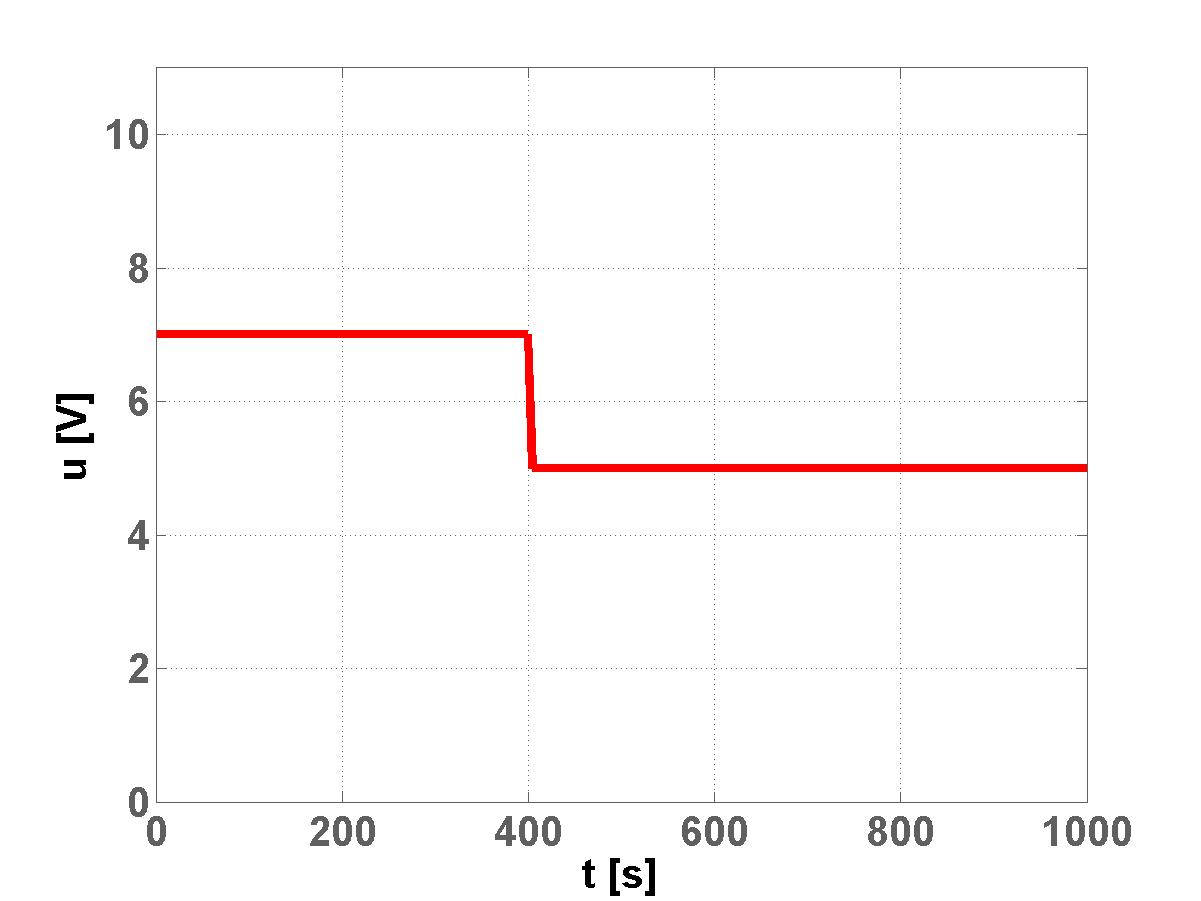
\includegraphics[width=6cm]{\cestaStyles Figures/Data_u}
  \caption{Obtékáný obrázek}
  \label{fig:Data_u2}
\end{center}
\end{wrapfigure}
V~tom pří\-pa\-dě dej\-te po\-zor na dě\-le\-ní slov. V~tom pří\-pa\-dě dej\-te po\-zor na dě\-le\-ní slov. V~tom pří\-pa\-dě dej\-te po\-zor na dě\-le\-ní slov. V~tom pří\-pa\-dě dej\-te po\-zor na dě\-le\-ní slov. V~tom pří\-pa\-dě dej\-te po\-zor na dě\-le\-ní slov. V~tom pří\-pa\-dě dej\-te po\-zor na dě\-le\-ní slov. V~tom pří\-pa\-dě dej\-te po\-zor na dě\-le\-ní slov. V~tom pří\-pa\-dě dej\-te po\-zor na dě\-le\-ní slov. V~tom pří\-pa\-dě dej\-te po\-zor na dě\-le\-ní slov. V~tom pří\-pa\-dě dej\-te po\-zor na dě\-le\-ní slov. V~tom pří\-pa\-dě dej\-te po\-zor na dě\-le\-ní slov. V~tom pří\-pa\-dě dej\-te po\-zor na dě\-le\-ní slov. V~tom pří\-pa\-dě dej\-te po\-zor na dě\-le\-ní slov. V~tom pří\-pa\-dě dej\-te po\-zor na dě\-le\-ní slov. V~tom pří\-pa\-dě dej\-te po\-zor na dě\-le\-ní slov. V~tom pří\-pa\-dě dej\-te po\-zor na dě\-le\-ní slov. V~tom pří\-pa\-dě dej\-te po\-zor na dě\-le\-ní slov. V~tom pří\-pa\-dě dej\-te po\-zor na dě\-le\-ní slov. V~tom pří\-pa\-dě dej\-te po\-zor na dě\-le\-ní slov. V~tom pří\-pa\-dě dej\-te po\-zor na dě\-le\-ní slov. V~tom pří\-pa\-dě dej\-te po\-zor na dě\-le\-ní slov. V~tom pří\-pa\-dě dej\-te po\-zor na dě\-le\-ní slov. V~tom pří\-pa\-dě dej\-te po\-zor na dě\-le\-ní slov. V~tom pří\-pa\-dě dej\-te po\-zor na dě\-le\-ní slov. V~tom pří\-pa\-dě dej\-te po\-zor na dě\-le\-ní slov. V~tom pří\-pa\-dě dej\-te po\-zor na dě\-le\-ní slov. V~tom pří\-pa\-dě dej\-te po\-zor na dě\-le\-ní slov. V~tom pří\-pa\-dě dej\-te po\-zor na dě\-le\-ní slov. V~tom pří\-pa\-dě dej\-te po\-zor na dě\-le\-ní slov. V~tom pří\-pa\-dě dej\-te po\-zor na dě\-le\-ní slov. V~tom pří\-pa\-dě dej\-te po\-zor na dě\-le\-ní slov. V~tom pří\-pa\-dě dej\-te po\-zor na dě\-le\-ní slov.


\subsection{Tabulky}

\begin{table}[H]
  \centering
  \caption{Obyčejná tabulka}\label{tab:values}
  \begin{tabular}{|l|c|r|}
    % after \\: \hline or \cline{col1-col2} \cline{col3-col4} ...
    \hline
    \textbf{Fyzikální veličina} & \textbf{Označení} & \textbf{Jednotka} \\ \hline
    {napětí na čerpadle}        & {$u$}             & {V}               \\ \hline
    {plocha podstavy nádrže}    & {$S$}             & {m$^2$}           \\ \hline
    {hustota}                   & {$\rho$}          & {kg\,m$^{-3}$}    \\ \hline
  \end{tabular}
\end{table}

\begin{table}[H]
  \centering
  \caption{Tabulka s dlouhými texty}\label{tab:text}
  \begin{tabular}{|p{9cm}|p{6cm}|}
    % after \\: \hline or \cline{col1-col2} \cline{col3-col4} ...
    \hline
    {co když je text v~1.~buňce strašně dlouhý, co když je text v~1.~buňce strašně dlouhý, co když je text v~1.~buňce strašně dlouhý}
        & {co když je text ve 2.~buňce strašně dlouhý}
        \\ \hline
    \parbox{5cm}{co když je text v~1.~buňce strašně dlouhý, co když je text v~1.~buňce strašně dlouhý, co když je text v~1.~buňce strašně dlouhý, co když je text v~1.~buňce strašně dlouhý, co když je text v~1.~buňce strašně dlouhý, co když je text v~1.~buňce strašně dlouhý, co když je text v~1.~buňce strašně dlouhý}
        & {co když je text ve 2.~buňce strašně dlouhý}
        \\ \hline
  \end{tabular}
\end{table}

\begin{table}[H]
  \catcode`\-=12
  \centering
  \caption{Tabulka se sloučenými buňkami}\label{tab:cells}
  \begin{tabular}{|l|c|c|}
    \hline
    {}                          & \multicolumn{2}{|c|}
                                    {\textbf{Fyzikální veličina}}       \\ \cline{2-3}
    \textbf{Popis}              & \textbf{označení} & \textbf{jednotka} \\ \hline
    {napětí na čerpadle}        & {$u$}             & {V}               \\ \hline
    {plocha podstavy nádrže}    & {$S$}             & {m$^2$}           \\ \hline
    {hustota}                   & {$\rho$}          & {kg\,m$^{-3}$}    \\ \hline
  \end{tabular}
\end{table}



\section{Křížové odkazy a~poznámky pod čarou}

Pro tvorbu křížových odkazů je třeba použít příkazy \verb"\label{}" a \verb"\ref{}", respektive pro citace příkaz
\verb"\cite{}", viz ná\-sle\-du\-jí\-cí příklady.

\begin{itemize}
    \item v~kapitole~\ref{ch:Uvod}
    \item Poznámky pod čarou se tvoří takto\footnote{Poznámka pod čarou je asi věta.}. Před číslem (horním indexem) není mezera.
    \item na~\figref{fig:ModelWS} nebo na~\figref{fig:Data_h}\footnote{Jak se píší poznámky pod čarou k~popisu obrázku se podívejte na~\figref{fig:Data}.}
    \item viz~\tabref{tab:values},
    \item podle rovnice~\eqref{eq:rovnice1},
    \item na literaturu, konkrétně
    \begin{itemize}
        \item na knihu~\cite{Book:ROUBAL-HUSEK-kol_RTvP},
        \item na část knihy~\cite[strana~10]{Book:ROUBAL-HUSEK-kol_RTvP}\footnote{Jak se cituje literatura v~popisu obrázku se podívejte
                na~\figref{fig:ModelWS}.},
        \item na článek v~časopise~\cite{Article:ROUBAL-HUSEK-STECHA_LSFOP},
        \item na web~\cite{WWW_Lab26},
        \item na diplomku~\cite{MastersThesis:ROUBAL_BP} nebo absolventské práce~\cite{AbsolventThesis:SIKYR_AP,AbsolventThesis:BOSTICKA_AP,AbsolventThesis:RABINAK_AP,AbsolventThesis:PAVLAT_AP},
    \end{itemize}
        seznam literatury je automaticky vygenerován za poslední kapitolou (před první přílohou),
    \item na definici~\ref{de:definice1}, větu~\ref{pr:veta1}, příklad~\ref{ex:priklad1}.
\end{itemize}



\section{Rovnice}

Rovnice je možné psát ručně přímo zde, nebo pomocí programu TeXaide, který je podobný editoru rovnic v~MS Word. Najdete ho zdarma na internetu.

Rovnice v~textu píšeme takto $y = 0\.5 x + 10$ (pozor na fonty, musí být stejné jako u~\uv{normálních} níže uvedených rovnic). V~\LaTeX\!\,u stačí dát výraz mezi dolary (\$ \$). Pro desetinnou čárku používáme \verb"\." -- jinak by se za čárkou objevila nežádoucí mezera podobně jako ve větách.


\subsection{Veličina, hodnota a fyzikální jednotka}

Fyzikální jednotky se nepíší kurzívou. Hodnota a~její jednotka se nesmí rozdělit na konci řádku. Správný zápis, se správně nastavenými mezerami mezi hodnotou a~jednotkou, je $u = 568\.3\,$mV. Což se TeXovsky zapíše takto
    \[
    \verb"$u = 568\.3\,$mV".
    \]


\subsection{Nečíslované rovnice}

    \[
    y = 0\.5 x + 10
    \]


\subsection{Číslované rovnice}

\begin{equation}\label{eq:rovnice1}
    y = 0\.5 x + 5
\end{equation}


\subsection{Maticové rovnice}

Maticové rovnice píšeme takto
\begin{equation}\label{eq:rovnice2}
    \mat{A} = \mat{B} + \mat{C},
\end{equation}
nebo takto
\begin{equation}\label{eq:rovnice3}
    \left[ \begin{array}{l}
        \dot x_1 (t) \\
        \dot x_2 (t) \\
    \end{array} \right] =
    \left[ {\begin{array}{*{20}c}
        1 & 1  \\
        0 & 2  \\
    \end{array}} \right]
    \left[ \begin{array}{l}
        x_1 (t) \\
        x_2 (t) \\
    \end{array} \right]\!.
\end{equation}
Nezapomeňte, že rovnice je součástí věty a~píšeme za ní čárky nebo tečky, jako v~nor\-mál\-ní slovní větě.



\section{Zdrojové kódy například z~Matlabu}

Takto je možné vkládat zdrojové kódy z~programovacích jazyků.
\begin{matlab}{.9\linewidth}{dgreen}
    %% Komentář ke kódu
    clc;
    clear;
    close all;

    omega = 1;
    jmn = [1 2*zeta*omega omega^2];

    figure(1);
        for zeta = 1E-5 : 0.2 : 1+1E-12
            G = tf(omega^2,subs([1 2*zeta*omega omega^2]));
            bode(G);
            hold on;
        end
        grid on;
    legend('\zeta = 0','\zeta = 0,2','\zeta = 0,4','\zeta = 0,6','\zeta = 0,8','\zeta = 1');
    text(1.1,230,'\infty','FontSize',16,'FontWeight','bold');
\end{matlab}
Pokud chcete změnit velikost písma, předefinujte jej v~příslušném souboru \texttt{\cestaStyles *.sty} na řádce~267.

Pokud chcete zachovat barvy kódu, pak použijte následující způsob. Podívejte se na zdrojový kód do souboru \texttt{\cestaStyles Manual\_tex.tex}. Pro změnu programovacího jazyka je nutno předefinovat v~příslušném souboru \texttt{\cestaStyles *.sty} na řádek~278.

\begin{lstlisting}
    %% Komentář ke kódu
    clc;
    clear;
    close all;

    omega = 1;
    jmn = [1 2*zeta*omega omega^2];

    figure(1);
        for zeta = 1E-5 : 0.2 : 1+1E-12
            G = tf(omega^2,subs([1 2*zeta*omega omega^2]));
            bode(G);
            hold on;
        end
        grid on;
    legend('\zeta = 0','\zeta = 0,2','\zeta = 0,4','\zeta = 0,6','\zeta = 0,8','\zeta = 1');
    text(1.1,230,'\infty','FontSize',16,'FontWeight','bold');
\end{lstlisting}



\section{Slova do rejstříku}


\index{Slovo do rejstříku 1}

\index{Slovo do rejstříku 2}

\index{charakteristika}

\index{charakteristika!přechodová}

\index{charakteristika!frekvenční}


Slova do rejstříku vkládáme pomocí klíčového slova \texttt{$\backslash$index\{\}}, do kterého napíšeme na patřičném místě v textu dané klíčové slovo, viz zdrojový text v~\texttt{\cestaStyles Manual\_tex.tex}.



\section{Definice, věty, příklady ...}

\begin{definition}[Název definice]\label{de:definice1}
Takto se píší definice.
\end{definition}

\begin{proposition}[Název věty]\label{pr:veta1}
Takto se píší věty.
\end{proposition}

\begin{example}[Název příkladu]\label{ex:priklad1}
Takto se píší příklady.
\end{example}
\begin{solution}
Takto je možné psát řešení příkladu.
\end{solution}

\begin{note}
Takto se píší poznámky.
\end{note}

\begin{proof}
Takto se píší důkazy.
\end{proof}



\textcolor{blue}{\em Tento text se nachází v~souboru \texttt{\cestaStyles Manual\_Tex.tex}. Pro odstranění této přílohy zakomentujte v~souboru \texttt{Diplomka.tex} řádek~170, respektive v~souboru \texttt{MP.tex} řádek~180, respektive v~souboru \texttt{SOC.tex} řádek~180\?: \texttt{$\backslash$input$\{$\cestaStyles Manual\_tex.tex$\}$}.\/}
           %input file
%\chapter{Citování a~formální náležitosti AP\label{ch:Manual_typo}}





Tato práce je napsána jako šablona pro absolventskou práci. Všimněte si zejména stylu dokumentu: zarovnání textu na obou stranách, popisy obrázků, číslování rovnic, číslování a~formátování kapitol, seznam literatury, odkazy na vztahy, obrázky atd.

V~toté příloze jsou shrnuta pravidla citování a~stručně uvedeny formální požadavky na práci spolu s~několika typografickými zásadami, které publikační systém \LaTeX\/ dodržuje sám. Více naleznete v~pří\-sluš\-ných normách. 



\section{Citování a~plagiátorství \label{se:Manual_cite}}

Využití cizích myšlenek upravuje citační etika a~normy! Nejprve ale uveďme základní pojmy, jako je citát, parafráze, citace a~citační odkaz~\cite{AbsolventThesis:FRANCIREK_AP}.
\begin{itemize}
    \item \textbf{Citát} je citovaná myšlenka nebo výrok jiného autora. Jde o~přímý a~doslovný přepis přebíraného obsahu.
    \item \textbf{Parafráze} je nepřímou variantou citátu. To znamená, že myšlenky jiného autora neopisujete doslovně, ale přepisujete je vlastními slovy.
    \item \textbf{Citace} neboli bibliografický záznam (zde je to kapitola Literatura) uvádí údaje o~citovaném zdroji (autory, název, místo vydání, rok vydání atd.).
    \item \textbf{Citační odkazy} spojují citáty či parafráze s~citacemi (zde je tvoříte příkazem \verb"\cite{}").
    \item \textbf{Plagiát} je dílo, ve kterém autor nepřizná použití cizích zdrojů. Jde o~neetické dílo odpovídající nezákonému obohacování se v~běžném životě.
    \item \textbf{Kompilát} je neužitečný přepis (byť i~správně citovaný) obsahu jiných děl po\-strá\-da\-jí\-cí váš přínos.
\end{itemize}

Tak, jak si můžete doslovně přečíst v~\cite{AbsolventThesis:FRANCIREK_AP}\?: \uv{Každá odborná práce stojí na dosavadním poznání těch, kteří se problematice věnovali před vámi, proto je využití jejich poznatků logické, žádoucí a~očekávané. Užitím citátů ukazujete, že znáte práce renomovaných odborníků, že na jejich práci navazujete a~že uznáváte jejich význam pro své vlastní poznání. Čtenáři umožňujete každý citát dohledat a~dozvědět se o~něm více.} Více si přečtěte v~\cite[kapitola~2.3.4]{AbsolventThesis:FRANCIREK_AP}.


\subsection{Několik rad k~citování}

\begin{itemize}
    \item \textbf{Je naprosto nepřípustné kopírovat cizí texty!} Samozřejmě, Ohmův zákon ne\-mů\-že\-te napsat jinak, než zní. Ale nesmíte spolu s~ním zkopírovat z~nějaké knihy či webové stránky celý odstavec nebo dokonce celou stránku (zákon včetně průvodních textů).
    \item Pokud používáte výsledky druhých autorů ve větším rozsahu, \textbf{je nepřípustné tupě kopírovat jejich texty.} Ty musíte parafrázovat a~opatřit je citačním odkazem. 
    \item Pokud je to bezpodmínečně nutné a~nějaká věta parafrázovat nelze (například proto, že by se ztratil nebo znepřesnil její význam), pak to lze vyřešit eticky následujícím způsobem. \textcolor{blue}{Jak autor/autoři ve své publikaci (konkrétní citační odkaz) uvádí\?: \uv{Tady bude zkopírovaná věta, maximálně krátký odstavec.}} Takto samozřejmě nelze zkopírovat každý druhý odstavec do Vaší AP.
\end{itemize}


\subsection{Relevantnost a~kvalita citací}

Obecně lze seřadit citační zdroje takto\?:
\begin{enumerate}
    \item \textbf{knihy}, zejména ty, které prošly kvalitním recenzním řízením (obvykle před rokem 2000) -- ne\-vý\-ho\-dou je samozřejmě jejich stáří, ale pokud jde o~základní učebnice, pak jsou to velmi kvalitní zdroje
    \item \textbf{články v~renomovaných časopisech} (zejména zahraničních) -- zde je výhoda v~jejich aktuálnosti a~vysoké odbornosti
    \item \textbf{články v~odborných časopisech}
    \item \textbf{články z~vědeckých konferencí}
    \item \textbf{diplomové práce}
    \item \textbf{absolventské/bakalářské práce}
    \item \textbf{odborná internetová fóra} -- pozor na kompetence autora
    \item \textbf{Wikipedie} -- tu necitujte, je velmi dobrá na první hledání, ale posléze je třeba najít informaci ve výše zmíněných zdrojích.
\end{enumerate}



\section{Shrnutí formálních požadavků}

\begin{enumerate}
    \item[1)] \emph{Srovnání textu}:
    \begin{enumerate}
        \item[a)] zarovnávejte text na obou stranách, vypadá to lépe;
        \item[b)] číslujte stránky;
        \item[c)] nevynechávejte volné půlstránky (čtvrtstránky), například pod obrázky (je to naprosto nepřípustné);
        \item[d)]  používejte odstavce v~rozumné míře (odstavec by měl mít více jak jednu větu, kapitola by měla mít více jak jeden odstavec atd.).
    \end{enumerate}
    \item[2)] \emph{Kapitoly}:
    \begin{enumerate}
        \item[a)] rozdělte práce přehledně do jednotlivých kapitol a~podkapitol, typicky: Úvod, pak kapitoly popisující problém, způsob Vašeho řešení, výsledky a~nakonec Závěr;
        \item[b)] číslujte kapitoly a~podkapitoly;
        \item[c)] použijte rozumné vertikální mezery kolem nadpisů kapitol.
    \end{enumerate}
    \item[3)] \emph{Rovnice a~matematika v~textu}:
    \begin{enumerate}
        \item[a)] rovnejte rovnice na střed, nebo na nějaký, stále stejný, tabulátor;
        \item[b)] číslujte rovnice, na které se odkazujete; číslování zarovnávejte zcela vpravo;
        \item[c)] matematika v~textu by měla být stejným stylem jako v~rovnicích (většinou kurzívou viz níže);
        \item[d)] fyzikální veličiny, například napětí \quantity{$u$}{V};
        \item[e)] fyzikální veličiny s~hodnotou, například $u=5\.4\,$V (všimněte si, jak napsat desetinnou čárku a~mezery mezi číslem a~jednotkou).
    \end{enumerate}
    \item[4)] \emph{Obrázky a~grafy}:
    \begin{enumerate}
        \item[a)] číslujte a~vhodně popisujte obrázky (například místo popisu frekvenční charakteristika napište hlavně čeho je to frekvenční charakteristika, jakého přenosu atd.);
        \item[b)] popisy obrázků zarovnávejte na střed nebo na nějaký, stále stejný, tabulátor;
        \item[c)] v~grafech popisujte česky (ne anglicky v~české práci) osy, přidejte legendy, vhodně zvolte tloušťku čar, nemíchejte dva neporovnatelné grafy (jablka, hruš\-ky), apod;
        \item[d)] nepoužívejte nekvalitně nascanované obrázky, nakreslete si je sami.
    \end{enumerate}
    \item[5)] \emph{Tabulky}:
    \begin{enumerate}
        \item[a)] podobně jako obrázky; popis většinou nad tabulku.
    \end{enumerate}
    \item[6)] \emph{Literatura}:
    \begin{enumerate}
        \item[a)] používejte odkazy na literaturu, nemusíte tak vysvětlovat spoustu pojmů;
        \item[b)] zdroj, na který se v~textu neodkazujete, nemá v~seznamu literatura co dělat;
        \item[c)] nadpis Literatura bývá obvykle bez čísla.
    \end{enumerate}
\end{enumerate}


Důraz klaďte na přehlednost, přesnost, stručnost a~ucelenost. Uvědomte si, že práci píšete i~pro někoho, kdo o~Vašem problému nemusí mít zdání! Popište tedy důkladně Váš problém. Popište, jak budete problém řešit a~jaké očekáváte řešení. Nesnažte se zakrýt tyto věci množstvím vzorečků a~okopírovaného textu z~internetu apod. Nejdůležitější kapitoly jsou úvod, kde je popsán problém a~závěr, kde shrnete Vaše výsledky. Porovnáte předpoklady se skutečností, vyhodnotíte všechny body zadání případně zdůvodníte proč jste některé body nevypracovali a~navrhnete možné řešení.

Práce nesmí na první pohled vypadat odpudivě, ale naopak poutavě. Jinak by si ji ni\-kdo nikdy nepřečetl a~i~vedoucí a~oponent ji bude číst s~předsudkem, že je to špatná práce! Práce by měla být i~slohově pěkná. Dejte ji přečíst někomu dalšímu a~pokud on ji dobře porozumí, je to dobrý základ proto, aby byla dobře ohodnocena. Také není od věci, nechat si práci jazykově a~gramaticky zkontrolovat nějakým odborníkem.



\section{Několik typografických zásad}

Čerpáno z~materiálů prof.~RNDr.~Petra Kulhánka,~CSc.\?: pravidla psaní výrazů. Sazba je určena mezinárodními normami (nemůžete psát texty, jak se Vám zlíbí)\?:
\begin{itemize}
    \item ISO\?: http://www.iso.ch/
    \item ČSN ISO\?: http://shop.normy.biz/
\end{itemize}

\noindent Sazba matematických výrazů\?:
\begin{itemize}
    \item normální (stojatá) sazba\?: pro čísla, funkce ($\sin,\, \cos$ apod.), číselné indexy, zkratky ($\max,\, \min$ apod.), jednotky (kg, N apod.), transpozici matice
    \item {\em italika (kurzíva)}\?: pro veličiny, proměnné, konstanty, indexy jako proměnné apod.
    \item \textbf{tučná sazba}\?: vektory, matice
    \item řecká písmena\?: proměnné italikou, suma apod. vyjádřená velkým řeckým Sigma normálním (stojatým) písmem
\end{itemize}

\noindent Mezery\?:
\begin{itemize}
    \item mezi číslem a~jednotkou (jednotky se nesmějí na konci řádku odělit od čísel)
    \item mezi jednotkami (1/4)
    \item před a~za rovnítkem
    \item argument funkce neuzavřený do závorky $(\sin 2x)$
    \item velikosti mezer v~matematice\?:
    \begin{itemize}
        \item \verb"\," 1/4
        \item \verb"\>" 1/2
        \item \verb"\;" 3/4
        \item \verb"\"  4/4 (celá)
        \item \verb"\quad"
        \item \verb"\qquad"
    \end{itemize}
    \item velikosti mezer v~textu\?:
    \begin{itemize}
        \item \verb"\," 1/4
        \item \verb"\/" italické vyrovnání
        \item \verb"\" 4/4 (celá)
        \item \verb"~" pevná
    \end{itemize}
\end{itemize}



\textcolor{blue}{\em Tento text se nachází v~souboru \texttt{\cestaStyles Manual\_typo.tex}. Pro odstranění této přílohy zakomentujte v~souboru \texttt{Diplomka.tex} řádek~171, respektive v~souboru \texttt{MP.tex} řádek~181, respektive v~souboru \texttt{SOC.tex} řádek~181\?: \texttt{$\backslash$input$\{$\cestaStyles Manual\_Typo.tex$\}$}.\/} 
          %input file
%\chapter{Finální formátování AP v~\LaTeXe \label{ch:Manual_final}}



Zde je popsáno finální formátování AP v \LaTeXe. Ponechte si na toto finální for\-má\-to\-vá\-ní cca \textcolor{red}{\textbf{20 dní}} (3~týdny na jazykovou korekturu, týden na formátovací korekturu) a~postupujte přesně podle následujícího návodu.

\begin{enumerate}
    \item Šablona pro AP je připravena pro oboustranný tisk, proto tolik bílých stran na začátku práce. Pokud chcete tisknout jednostranně, odkomentujte v~souboru {\rm \texttt{Diplomka.tex}} řádek~1 a zakomentujte řádek~2.
    \item Pokud nechcete mít v~práci Rejstřík, odkomentujte v~souboru {\rm \texttt{Diplomka.tex}} řádky~179 a~185, respektive v~souboru \texttt{MP.tex} řádky~189 a~195, respektive v~souboru \texttt{SOC.tex} řádky~189 a~195\?: $\backslash$\texttt{iffalse} a~$\backslash$\texttt{fi}.
    \item Pokud jste provedli přesně a~všechny tamní pokyny, \textcolor{blue}{\em vymažte barevný text v~souboru \newline \texttt{00\_files/Task.tex}.}
    \item Pokud jste provedli přesně a~všechny tamní pokyny, \textcolor{blue}{\em vymažte barevný text v~souboru \newline \texttt{00\_files/Deklar.tex}.}
    \item Vraťte se k~poděkování a~nezapomeňte poděkovat těm, kteří Vám s~prací pomáhali (byla to jejich dobrá vůle), svým blízkým za podporu při studiu, případně škole za finanční podporu Vašeho projektu atd. \textbf{Je naprosto nevhodné někomu poděkovat například za jazykovou korekturu a~pak mít v~práci gramatické chyby apod.} Dejte na to prosím pozor.
    \item Vraťte se k~anotaci a~zkontrolujte, že obsahuje to, co obsahovat má.
    \item Zkontrolujte, že je dobře naformátovaný obsah práce, seznam obrázků, seznam tabulek a~záhlaví stránek.
    \begin{itemize}
        \item Pokud jsou některé texty v~těchto částech práce příliš dlouhé, použijte alternativní zápis
            \begin{center}
                \verb"\chapter[Zkrácený název]{Původní (dlouhý) název}",
                \verb"\section[Zkrácený název]{Původní (dlouhý) název}",
                \verb"\caption[Zkrácený název]{Původní (dlouhý) název}".
            \end{center}
    \end{itemize}
    \item Pokud jste provedli přesně a~všechny tamní pokyny, \textcolor{blue}{\em vymažte barevný text v~souboru \newline \texttt{00\_files/Symbols.tex}, respektive \texttt{00\_files/Abbreviation.tex}.}
    \item \textcolor{red}{Vraťte se k~úvodu práce a~zkontrolujte, že obsahuje \textbf{motivaci}, \textbf{stav řešeného pro\-blé\-mu}, \textbf{cíl práce} a \textbf{strukturu práce}, dle pokynů v~kapitole~\ref{ch:Uvod}.}
    \item \textcolor{blue}{\em Zkontrolujte sazbu literatury a~její abecední řazení. Poté odkomentujte v~souboru \texttt{Diplomka.tex} řádky 152 a~154, respektive v~souboru \texttt{MP.tex} řádky~152 a~154, respektive v~souboru \texttt{SOC.tex} řádky~152 a~154 \?: $\backslash$\texttt{iffalse} a~$\backslash$\texttt{fi}.}
    \item Vložte pevné (nerozdělitelné) mezery tam, kde mají být (tj. za jednopísmenné před\-lož\-ky, mezi titul a~jméno atd.).
    \begin{itemize}
        \item V~\LaTeX\,\!u je to pomocí symbolu $\sim$. K~vložení symbolu $\sim$ k~jednopísmenným předložkám lze použít skript \verb"vlnka.bat", který spustíte s~parametrem pří\-sluš\-né\-ho \verb"*.tex" souboru.
    \end{itemize}
    \item Zkontrolujte, že nemáte na stránkách vynechaná \textcolor{red}{bílá místa} (vyjma posledních strá\-nek příslušných kapitol). \textcolor{red}{Je to nepřípustné!!!}
    \item Zkontrolujte dělení slov v~celé práci.
    \begin{itemize}
        \item Připište do prvního respektive druhého řádku souboru \texttt{Diplomka.tex}, respektive souboru \texttt{MP.tex}, respektive souboru \texttt{SOC.tex} do hranatých závorek parametr \verb"draft" a~klikněte ve \hbox{WinEDT} na ikonu \verb"TeXify" (med\-ví\-dek ve verzi~5.3). Pokud bude nějaké slovo špatně rozděleno, objeví se v~DVI souboru na příslušném místě černý obdélníček. Dělení slov opravíte pomocí \verb"\-".
        \item Vymažte v~souboru \texttt{Diplomka.tex}, respektive souboru \texttt{MP.tex}, respektive souboru \texttt{SOC.tex} parametr \verb"draft".
    \end{itemize}
    \item Klikněte ve WinEDT na ikonu \verb"koš" a~vymažte všechny dočasné soubory. Poté klik\-ně\-te ve WinEDT na ikonu \verb"TeXify" (medvídek ve verzi~5.3), čímž se vytvoří \uv{finální} DVI soubor. Následně otevřete soubor \verb"Diplomka.log", respektive soubor \texttt{MP.log}, respektive soubor \texttt{SOC.log} a~vyhledejte v~něm slova
        \begin{center}
            \verb"undefined",\\
            \verb"multiply".
        \end{center}
        Pokud jste nějaká taková slova našli, znamená to, že některý \verb"label" neexistuje respektive je duplicitní. Toto opravte a~zopakujte tento bod.
    \item \textcolor{blue}{\em Vymažte zbylé barevné texty z~ostatních souborů a~zakomentujte v~\texttt{Diplomka.tex} řádky~170 až~171, respektive v~\texttt{MP.tex} řádky~180 až~181, respektive v~\texttt{SOC.tex} řádky~180 až~181. Dále zakomentujte v~\texttt{Diplomka.tex} přílohy, které nechcete ve své práci mít (řádky~168 až~169).}
    \item Až budete mít vyrobené desky pro absolventksou práci, odkomentujte v~souboru {\rm \texttt{Diplomka.tex}} řádky~52 {\rm $\backslash$\texttt{iffalse}} a~65 {\rm $\backslash$\texttt{fi}}. Tím tyto desky a~volné stránky z~výsledného PDF zmizí.
    \item Vymažte všechny "*.bak" soubory.
    \item \textcolor{brown}{Klikněte ve WinEDT na ikonu {\rm \texttt{koš}} a~vymažte všechny dočasné soubory. Poté klik\-ně\-te ve WinEDT na ikonu {\rm \texttt{TeXify}} (medvídek ve verzi~5.3), čímž se vytvoří finální DVI soubor. Následně klikněte ve WinEDT na ikonu {\rm \texttt{dvipdf}}, čímž se vytvoří finální PDF soubor.}
    \item Dejte práci k~češtinářské korektuře a~proveďte příslušné opravy.
    \item \textcolor{dgreen}{\em Zakomentujte v~souboru \texttt{Diplomka.tex} řádek~172 (v~souboru \texttt{MP.tex}, respektive \texttt{SOC.tex} řá\-dek~182). Dále změňte v~\texttt{Diplomka.tex}, respektive \texttt{MP.tex}, respektive \texttt{SOC.tex} na řádku~22 obsah proměnné \texttt{$\backslash$APforPrint} na hodnotu~1. Zopakováním bodu 18 tohoto návodu vygenerujete výsledné PDF pro tisk.}
    \item \textcolor{dgreen}{\em Změňte v~souboru \texttt{Diplomka.tex}, respektive \texttt{MP.tex}, respektive \texttt{SOC.tex} na řádku 22 obsah pro\-měn\-né \texttt{$\backslash$APforPrint} zpět na hodnotu~0. Zopakováním bodu 18 tohoto návodu vygenerujete výsledné PDF pro CD/DVD a~MOODLE.}
\end{enumerate}


\textcolor{blue}{\em Tento text se nachází v~souboru \texttt{\cestaStyles Manual\_final.tex}. Pro odstranění této pří\-lo\-hy zakomentujte v~\texttt{Diplomka.tex} řádek 172 (v~souboru \texttt{MP.tex}, respektive \texttt{SOC.tex} řádek~182)\?: \newline \texttt{$\backslash$input$\{$\cestaStyles Manual\_final.tex$\}$}.\/} 
         %input file
\end{appendix}
%-----<<< --------- >>>-----



%-----<<< INDEX >>>-----
% NECHCI TVUJ SPINAVEJ RESTRIK
\iffalse
\cleardoublepage \addcontentsline{toc}{chapter}{Rejstřík}
\printindex

\textcolor{blue}{\em Tento text se nachází v~souboru\/ {\rm\texttt{Diplomka.tex} na řádcích 179-185}. Pro odstranění rejstříku, odkomentujte v~souboru {\rm \texttt{Diplomka.tex}} řádky 179\?: $\backslash$\texttt{iffalse} a~185\?: $\backslash$\texttt{fi}.\\[2ex] Pokud chcete vkládat klíčová slova do rejstříku, používejte příkaz $\backslash$\texttt{index\{\}}.}
\fi
%-----<<< ----- >>>-----

\end{document}
%-----<<<<<<<<< END OF DOCUMENT >>>>>>>>>----- 
